\documentclass[a4paper, 12pt]{article}
\usepackage[a4paper,top=1.5cm, bottom=1.5cm, left=1cm, right=1cm]{geometry}
\usepackage[utf8]{inputenc}
\usepackage{mathtext}
\usepackage{amsmath}
\usepackage{amsfonts}
\usepackage[english, russian]{babel}
\usepackage{indentfirst}
\usepackage{longtable}
\usepackage{graphicx}
\graphicspath{{pictures/}}
\DeclareGraphicsExtensions{.pdf,.png,.jpg}
\usepackage{natbib}
\usepackage{mathrsfs}

\title{Лабораторная работа 1.2.5 Исследование вынужденной регулярной прецессии гироскопа}
\author{Михаил Колтаков}
\date{5 октября 2020 г.}

\begin{document}
	\maketitle
	\section*{Цель работы}
		Исследовать вынужденную прецессию гироскопа; установить зависимость скорости вынужденной прецессии от величины момента сил, действующих на ось гироскопа; определить скорость вращения ротора гироскопа и сравнить её со скоростью, рассчитанной по скорости прецессии.
	\section*{Оборудование}
		Гироскоп в карданном подвесе, секундомер, набор грузов, отдельный ротор гироскопа, цилиндр известной массы и диаметра, крутильный маятник, штангенциркуль, линейка.
	\section*{Теория к работе}
		Уравнения движения твёрдого тела можно записать в виде
		\begin{equation}
			\label{Force}
			\frac{d \vec{P}}{dt} = \vec{F}
		\end{equation}
		\begin{equation}
			\label{Torque}
			\frac{d \vec{L}}{dt} = \vec{M}
		\end{equation}
		Здесь (\ref{Force}) выражает закон движения центра масс тела, а (\ref{Torque}) -- уравнение моментов. Если сила $\vec{F}$ не зависит от угловой скорости, а момент сил $\vec{M}$ -- от скорости поступательного движения, то уравнения (\ref{Force}) и (\ref{Torque}) можно рассматривать независимо. В нашем случае так и происходит, поэтому для описания движения гироскопа потребуется только уравнение (\ref{Torque}).
		Момент импульса вращающегося твёрдого тела можно выразить по формуле
		$$\vec{L} = \vec{i} I_x \omega_x + \vec{j} I_y \omega_y  + \vec{k} I_z \omega_z,$$
		где $I_x, I_y, I_z$ -- главные моменты инерции, а $\omega_x, \omega_y, \omega_z$ -- компоненты вектора угловой скорости $\vec{\omega}$. Если произведение момента по какой-то оси на компоненту угловой скорости по этой же оси много больше, чем другие такие произведения, то такое вращающееся тело называется гироскопом.
		\par
		Приращение момента импульса можно выразить по формуле
		$$ \Delta \vec{L} = \int \vec{M} dt$$
		Если момент внешних сил прикладывается в течение короткого промежутка времени, то из интеграла следует, что $|\Delta \vec{L}| \ll |\vec{L}|$. С этим связана устойчивость гироскопа после приведения его в быстрое вращение.
		\par
		Если к оси гироскопа прикладывать небольшой момент силы, то он будет вращаться с угловой скоростью $\Omega$, и при этом $L_\Omega \ll L_{\omega_0}$, где $\omega_0$ -- угловая скорость вращения гироскопа в основном направлении.
		\par
		Из этого можно вывести формулу
		$$ \frac{d \vec{L}}{dt} = \vec{M} = \vec{\Omega} \times \vec{L} $$
		Из этого уравнения можно вывести уравнение для угловой скорости прецессии $\Omega$ с учётом массы подвешенных грузов и расстояния до них.
		$$\Omega = \frac{m g l}{I_z \omega_0}$$
		$m$ - масса груза,
		$l$ - расстояние от центра карданного подвеса до точки подвеса груза,
		$I_z$ - момент инерции гироскопа относительно основной оси вращения,
		$\omega_0$ - угловая скорость вращения гироскопа относительно основной оси вращения(скорость вращения вала мотора)
		\par
		Момент инерции $I_z$ можно рассчитать с помощью крутильного маятника, подвесив к нему сначала цилиндр известной массы и диаметра, т.е. момент которого мы знаем, а потом гироскоп. Тогда
		$$ I_z = I_ц \frac{T_z^2}{T_ц^2} $$
		$T_ц - период\: крутильных\: колебаний\: цилиндра,\: а\: T_z - период\: крутильных\: колебаний\: гироскопа$
	\section*{Ход работы}
		\thispagestyle{empty}
		Проведём измерения для грузов 5 различных масс, проведя по 5 измерений для каждой массы и занесём результаты измерений в таблицу.
		\begin{longtable}[H]{|c|c|c|c|c||c|c|c|}
			\hline
			$m,\: г$ & $T,\: с$ & Кол-во оборотов & $\Omega \cdot 10^{2},\: \frac{рад}{с} $ & $\overline{\Omega} \cdot 10^{2},\: \frac{рад}{с}$ & $Верт.\: \angle, рад$ & $\Omega_{\mu} \cdot 10^3\: \frac{рад}{с}$ & $\overline{\Omega_{\mu}} \cdot 10^{3},\: \frac{рад}{с}$ \\
			\hline
			& 335 & 4 & 7,6 &  & 0,46 & 1,4 &  \\
			& 329 & 4 & 7,4 &  & 0,44 & 1,4 &  \\
			142 & 333 & 4 & 7,6 & 7,6 & 0,46 & 1,4 & 1,4 \\
			& 331 & 4 & 7,5 &  & 0,42 & 1,3 &  \\
			& 322 & 4 & 7,8 &  & 0,43 & 1,3 &  \\
			\hline
			& 272 & 4 & 9,3 &  & 0,45 & 1,6 &  \\
			& 269 & 4 & 9,2 &  & 0,45 & 1,7 &  \\
			176 & 271 & 4 & 9,3 & 9,3 & 0,45 & 1,6 & 1,6 \\
			& 274 & 4 & 9,4 &  & 0,46 & 1,6 &  \\
			& 272 & 4 & 9,3 &  & 0,46 & 1,7 &  \\
			\hline
			& 273 & 5 & 11,6 &  & 0,57 & 2,0 &  \\
			& 271 & 5 & 11,6 &  & 0,58 & 2,1 &  \\
			220 & 269 & 5 & 11,5 & 11,6 & 0,58 & 2,0 & 2,0 \\
			& 275 & 5 & 11,7 &  & 0,57 & 2,0 &  \\
			& 270 & 5 & 11,5 &  & 0,57 & 2,0 &  \\
			\hline
			& 222 & 5 & 14,4 &  & 0,57 & 2,5 &  \\
			& 219 & 5 & 14,3 &  & 0,58 & 2,6 &  \\
			273 & 220 & 5 & 14,3 & 14,3 & 0,58 & 2,6 & 2,6 \\
			& 217 & 5 & 14,2 &  & 0,57 & 2,5 &  \\
			& 224 & 5 & 14,4 &  & 0,58 & 2,6 &  \\
			\hline
			& 213 & 6 & 17,7 &  & 0,70 & 3,3 &  \\
			& 210 & 6 & 17,5 &  & 0,68 & 3,2 &  \\
			342 & 214 & 6 & 17,8 & 17,7 & 0,70 & 3,3 & 3,3 \\
			& 212 & 6 & 17,6 &  & 0,69 & 3,3 &  \\
			& 216 & 6 & 17,9 &  & 0,70 & 3,3 &  \\
			\hline
		\end{longtable}
		Для каждого грузика можно рассчитать момент, который он создаёт по формуле $\vec{M} = ml \vec{g}$
		\par
		Оценим погрешность измерения $\Omega$:
		Массы грузов и длина рычага измерены очень точно, поэтому их погрешностью можно пренебречь, значит, моменты сил измерены без погрешностей.
		Погрешность измерения времени с помощью секундомера - 0,2с.
		Можем рассчитать угловую скорость вращения вала мотора в гироскопе по формуле
		$$\omega_0 = \frac{mgl}{I_z \Omega} \;\;\;\;\;\;\; \omega_0 \sim \frac{M}{\Omega}$$
		Выходит, искомую угловую скорость можно рассчитать как коэффициент угла наклона графика $M(\Omega)$(график в конце работы, кресты погрешностей настолько малы, что ложатся внутри точек)
		\par
		Рассчитаем момент инерции цилиндра из его массы $m_ц = 1617,8 \pm 0,2г$ и диаметра $d_ц = 78,1 \pm 0,1мм$.
		$$I_ц = \frac{m_ц d_ц^2}{8} \approx 1,2 \cdot 10^{-3}\: кг \cdot м^2$$ \\
		Погрешности измерения $T_ц\: и\: T_0 = 0,2 с$
		\thispagestyle{empty}
		\begin{longtable}[H]{|c|c||c|c|}
			\hline
			$t_ц,\: с$ & Кол-во периодов & $t_0,\: с$ & Кол-во периодов \\
			\hline
			46,5 & 10 & 17,9 & 5 \\
			\hline
			44,7 & 10 & 17,5 & 5 \\
			\hline
			44,6 & 10 & 17,6 & 5 \\
			\hline
			45,1 & 10 & 18,2 & 5 \\
			\hline
			45,2 & 10 & 17,5 & 5 \\
			\hline
		\end{longtable}
		\thispagestyle{plain}
		Среднее значение $T_ц = 4,5\: с$, а среднее значение $T_0 = 3,5\: с$
		Тогда можно определить
		$$I_0 = I_ц \frac{T_0^2}{T_ц^2} =\frac{3,5^2}{4,5^2} \cdot 1.2 \cdot 10^{-3} = 0,73 \cdot 10^{-3}\: кг \cdot м^2$$
		Погрешность при измерении $I_0\: равна\: 0,02 \cdot 10^{-3}\: кг \cdot м^2$.
		Относительная погрешность при измерении угловой скорости прецессии $\Omega$ имеет порядок $10^{-3}$, поэтому ей можно пренебречь.
		Рассчитаем частоту вращения гироскопа по формуле, указанной выше
		\begin{longtable}[H]{|c|c|c|c|c|c|}
			\hline
			Масса груза, г & 142 & 176 & 220 & 273 & 342 \\
			\hline
			$\omega_0,\: рад/c$ & 3065 & 3098 & 3086 & 3102 & 3123 \\
			\hline
		\end{longtable}
		Усреднив, получим $\overline{\omega_0} = 3095 \pm 28\: рад/с$, тогда частота будет равна $\nu_0 = 492,6 \pm 4,5\: Гц$.
		\par
		Оценим действие силы трения по скорости опускания рычага
		$$M_{тр}=F_{тр} l= \frac{m \Omega_{\mu} l^2}{t}$$
		$$L_{тр} = M_{тр} t$$
		При вычислении точных значений моментов силы трения получаются величины порядка $10^{-8}$, а при вычислении моментов импульса силы трения получаются величины порядка $10^{-6}$. И то, и другое значения много меньше других, поэтому ими можно пренебречь в расчётах.
		\par
		Другим методом измерения скорости вращения вала мотора является получение стабильного эллипса на экране осцилографа, подключив его к второй обмотке статора гироскопа и к генератору синусоидальных сигналов. Этим методом мы получаем значение $\nu_{осц} = 490,3 Гц$, погрешностью измерения которого можно пренебречь. 
		Это значение лежит в пределах $0,5\%$ от определённого с помощью подвешивания грузов.
	\section*{Вывод}
		При измерении угловой скорости двумя разными методами результаты совпали с точностью $0,5\%$. Теория согласуется с практикой, небольшие расхождения можно объяснить трением в осях карданного подвеса, хотя и его момент много меньше моментов других сил. Гипотеза о том, что $L_{\Omega} \ll L_{\omega_0}$ подтвердилась. В итоге угловую скорость мотора гироскопа можно считать равной $3095 \pm 28 рад/с$.
	\begin{figure}[h!]
		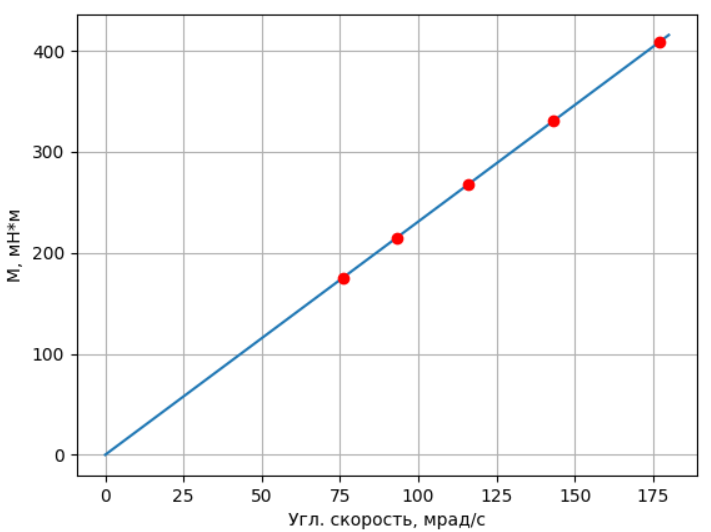
\includegraphics[width=\linewidth]{pict1}
	\end{figure}
\end{document}
